\documentclass[11pt,a4paper]{article}

\usepackage[T1]{fontenc}
\usepackage[utf8]{inputenc}
\usepackage{lmodern}
\usepackage[french]{babel}
\usepackage{amsmath,amssymb,amsthm}
\usepackage[margin=2.4cm]{geometry}
\usepackage{graphicx}
\usepackage{booktabs}
\usepackage{float}
\usepackage[font=small,labelfont=bf]{caption}
\usepackage{microtype}
\usepackage{xcolor}
\usepackage[colorlinks=true,linkcolor=violet,urlcolor=violet,citecolor=violet]{hyperref}

% Generated by experiments/run_all.py: do not edit by hand.

\newcommand{\tableStationary}{%
Système linéaire (Gauss) & $1{,}9 \times 10^{-16}$ & -- & 1{,}3 \\
Puissance (chaîne paresseuse) & $1{,}5 \times 10^{-14}$ & 297 itérations & 2{,}1 \\
Simulation (fréquences) & $7{,}2 \times 10^{-4}$ & 1\,000\,000 pas & 2072{,}2 \\
}
\newcommand{\nSim}{1\,000\,000}
\newcommand{\powIters}{297}
\newcommand{\tableGap}{%
Cycle, $m = 10$ & 0{,}904508 & 0{,}904508 & 10 \\
Cycle, $m = 20$ & 0{,}975528 & 0{,}975528 & 38 \\
Cycle, $m = 40$ & 0{,}993844 & 0{,}993844 & 152 \\
Ehrenfest paresseuse, $N = 20$ & 0{,}950000 & 0{,}950003 & 39 \\
Ehrenfest paresseuse, $N = 50$ & 0{,}980000 & 0{,}980001 & 120 \\
}
\newcommand{\mixSlope}{2{,}00}
\newcommand{\mixHundred}{1555}
\newcommand{\nAirports}{3\,425}
\newcommand{\nRoutes}{37\,594}
\newcommand{\nRouteEntries}{67\,662}
\newcommand{\nDangling}{16}
\newcommand{\prIters}{169}
\newcommand{\diffNX}{6{,}6 \times 10^{-13}}
\newcommand{\timeOurs}{78}
\newcommand{\timeNX}{239}
\newcommand{\spearmanDeg}{0{,}807}
\newcommand{\algRank}{139}
\newcommand{\algDegRank}{185}
\newcommand{\algScore}{1{,}33 \times 10^{-3}}
\newcommand{\uniformScore}{2{,}92 \times 10^{-4}}
\newcommand{\nSCC}{44}
\newcommand{\largestSCC}{3\,354}
\newcommand{\nClosed}{7}
\newcommand{\closedSizes}{10, 4, 4, 4, 2, 2, 2}
\newcommand{\tableTop}{%
1 & \texttt{ATL} & Atlanta (\'Etats-Unis) & 9{,}312 & 1 \\
2 & \texttt{ORD} & Chicago (\'Etats-Unis) & 5{,}861 & 2 \\
3 & \texttt{LAX} & Los Angeles (\'Etats-Unis) & 5{,}654 & 6 \\
4 & \texttt{DFW} & Dallas-Fort Worth (\'Etats-Unis) & 5{,}375 & 8 \\
5 & \texttt{CDG} & Paris (France) & 4{,}943 & 5 \\
6 & \texttt{LHR} & Londres (Royaume-Uni) & 4{,}942 & 4 \\
7 & \texttt{SIN} & Singapour (Singapour) & 4{,}816 & 12 \\
8 & \texttt{PEK} & P\'ekin (Chine) & 4{,}811 & 3 \\
9 & \texttt{DEN} & Denver (\'Etats-Unis) & 4{,}754 & 14 \\
10 & \texttt{FRA} & Francfort (Allemagne) & 4{,}516 & 7 \\
11 & \texttt{JFK} & New York (\'Etats-Unis) & 4{,}455 & 9 \\
12 & \texttt{DME} & Moscou (Russie) & 4{,}379 & 26 \\
13 & \texttt{AMS} & Amsterdam (Pays-Bas) & 4{,}153 & 10 \\
14 & \texttt{MIA} & Miami (\'Etats-Unis) & 4{,}110 & 16 \\
15 & \texttt{IST} & Istanbul (Turquie) & 4{,}107 & 17 \\
}
\newcommand{\tableUp}{%
\texttt{FAI} & Fairbanks (\'Etats-Unis) & 86 & 507 \\
\texttt{BET} & Bethel (\'Etats-Unis) & 71 & 488 \\
\texttt{ANC} & Anchorage (\'Etats-Unis) & 43 & 273 \\
\texttt{AEP} & Buenos Aires (Argentine) & 55 & 259 \\
\texttt{THR} & T\'eh\'eran (Iran) & 97 & 264 \\
}
\newcommand{\slopeErgodic}{-0{,}51}
\newcommand{\nChains}{400}
\newcommand{\slopeMC}{-0{,}48}
\newcommand{\errMCmillion}{0{,}039}
\newcommand{\sameTopTen}{10}
\newcommand{\tableMC}{%
1\,000 & 1{,}0533 & 0{,}01 \\
3\,000 & 0{,}7144 & 0{,}01 \\
10\,000 & 0{,}3915 & 0{,}02 \\
30\,000 & 0{,}2207 & 0{,}04 \\
100\,000 & 0{,}1217 & 0{,}13 \\
300\,000 & 0{,}0734 & 0{,}39 \\
1\,000\,000 & 0{,}0392 & 1{,}35 \\
}
\newcommand{\itersEightyFive}{104}
\newcommand{\boundEightyFive}{142}
\newcommand{\msPerIter}{0{,}33}
\newcommand{\tableAlpha}{%
0{,}50 & 0{,}4654 & 26 & 33 \\
0{,}70 & 0{,}6717 & 49 & 64 \\
0{,}85 & 0{,}8343 & 104 & 142 \\
0{,}95 & 0{,}9449 & 308 & 451 \\
0{,}99 & 0{,}9900 & 1597 & 2311 \\
}


\newtheorem{proposition}{Proposition}
\newtheorem{theoreme}{Théorème}
\newtheorem{definition}{Définition}
\theoremstyle{remark}
\newtheorem*{remarque}{Remarque}

\newcommand{\R}{\mathbb{R}}
\newcommand{\E}{\mathbb{E}}
\newcommand{\1}{\mathbf{1}}
\newcommand{\TV}{\mathrm{TV}}
\newcommand{\PP}{\mathbb{P}}

\title{\textbf{Chaînes de Markov et PageRank :\\ de la théorie au réseau aérien mondial}}
\author{Yassine Abderrezak Dache\\[2pt]\small Projet personnel \textendash{} Python (NumPy, Matplotlib)\\[1pt]\small\url{https://github.com/yassinedache/markov-chains-pagerank}}
\date{\today}

\begin{document}
\maketitle

\begin{abstract}
On étudie les chaînes de Markov à espace d'états fini et l'une de leurs applications les plus connues, l'algorithme PageRank. La loi stationnaire est calculée de trois façons programmées sans bibliothèque spécialisée (système linéaire résolu par élimination de Gauss, itération de la puissance, simulation), et l'on vérifie expérimentalement les résultats théoriques sur la vitesse de convergence : la distance à l'équilibre décroît exactement au rythme de la deuxième valeur propre, et le temps de mélange de la marche sur un cycle de $m$ sites croît comme $m^{\mixSlope}$ (théorie : $m^2$). PageRank est ensuite appliqué au réseau aérien mondial (\nAirports{} aéroports, \nRoutes{} liaisons) : la méthode de la puissance, dont on démontre la convergence en $\alpha^k$, retrouve les scores de NetworkX à $\diffNX$ près, et un estimateur de Monte-Carlo fondé sur des marches aléatoires converge en $1/\sqrt N$ comme prévu.
\end{abstract}

\section{Chaînes de Markov finies}

\begin{definition}
Soit $E = \{1, \dots, n\}$ et $P \in \R^{n\times n}$ une matrice \emph{stochastique} : $P_{ij} \ge 0$ et $\sum_j P_{ij} = 1$. Une suite de variables aléatoires $(X_k)_{k\ge0}$ à valeurs dans $E$ est une chaîne de Markov de matrice de transition $P$ si
\[
  \PP(X_{k+1} = j \mid X_k = i,\, X_{k-1}, \dots, X_0) = P_{ij}.
\]
\end{definition}

On note $\mu_k$ la loi de $X_k$, vue comme un vecteur ligne. La formule des probabilités totales donne $\mu_{k+1} = \mu_k P$, donc $\mu_k = \mu_0 P^k$. Une loi $\pi$ est \emph{stationnaire} si $\pi P = \pi$ : c'est un vecteur propre à gauche de $P$ pour la valeur propre $1$.

La chaîne est \emph{irréductible} si tout état peut être atteint depuis tout autre ; la \emph{période} d'un état $i$ est le pgcd des longueurs des chemins de $i$ à $i$ (elle est la même pour tous les états d'une chaîne irréductible), et la chaîne est \emph{apériodique} si elle vaut $1$. On rappelle les deux théorèmes fondamentaux, démontrés par exemple dans \cite{norris,lpw}.

\begin{theoreme}[convergence et théorème ergodique]\label{thm:fond}
Une chaîne irréductible sur un ensemble fini possède une unique loi stationnaire $\pi$, et $\pi_i > 0$ pour tout $i$.
\begin{enumerate}
\item \emph{(Théorème ergodique)} Pour toute loi initiale, la proportion du temps passé en $i$ converge presque sûrement : $\frac1n \sum_{k=0}^{n-1} \1_{\{X_k = i\}} \to \pi_i$.
\item \emph{(Convergence en loi)} Si de plus la chaîne est apériodique, $\mu_k \to \pi$ pour toute loi initiale $\mu_0$.
\end{enumerate}
\end{theoreme}

\begin{proposition}[équilibre détaillé]\label{prop:reversible}
Si une loi $\pi$ vérifie $\pi_i P_{ij} = \pi_j P_{ji}$ pour tous $i, j$, alors $\pi$ est stationnaire. On dit alors que la chaîne est \emph{réversible}.
\end{proposition}

\begin{proof}
$(\pi P)_j = \sum_i \pi_i P_{ij} = \sum_i \pi_j P_{ji} = \pi_j \sum_i P_{ji} = \pi_j$.
\end{proof}

\begin{remarque}
La chaîne \emph{paresseuse} $Q = \frac12 (I + P)$ reste sur place avec probabilité au moins $\frac12$. Elle a les mêmes lois stationnaires que $P$, elle est apériodique puisque $Q_{ii} > 0$, et ses valeurs propres sont les $\frac{1+\lambda}{2}$ pour $\lambda$ valeur propre de $P$. C'est l'outil standard pour supprimer la périodicité.
\end{remarque}

\section{L'urne d'Ehrenfest : trois calculs de la loi stationnaire}

Le modèle d'Ehrenfest (1907), introduit pour illustrer la diffusion d'un gaz entre deux compartiments, contient $N$ boules réparties entre deux urnes $A$ et $B$. À chaque étape, on choisit une boule au hasard et on la change d'urne. L'état est le nombre $k$ de boules dans $A$ :
\[
  P_{k,k-1} = \frac kN, \qquad P_{k,k+1} = \frac{N-k}{N}.
\]

\begin{proposition}
La loi stationnaire est la loi binomiale $\mathcal B(N, \frac12)$ : $\pi_k = \binom Nk 2^{-N}$. La chaîne est de période $2$.
\end{proposition}

\begin{proof}
On vérifie l'équilibre détaillé :
\[
  \pi_k P_{k,k+1} = \binom Nk \frac{N-k}{N}\, 2^{-N} = \binom N{k+1} \frac{k+1}{N}\, 2^{-N} = \pi_{k+1} P_{k+1,k},
\]
car $\binom Nk (N-k) = \binom N{k+1}(k+1) = \frac{N!}{k!\,(N-k-1)!}$. À chaque pas, $k$ change de $\pm1$, donc sa parité alterne : un retour en $k$ demande un nombre pair d'étapes, et $k \to k+1 \to k$ en demande $2$.
\end{proof}

La loi binomiale est donc connue exactement, ce qui permet de mesurer l'erreur de trois méthodes de calcul (avec $N = 20$, soit $21$ états).

\paragraph{Système linéaire.} Les $n$ équations $\pi(P - I) = 0$ sont liées (leur somme est nulle) ; pour une chaîne irréductible le noyau est de dimension $1$, et l'on remplace la dernière équation par la normalisation $\sum_i \pi_i = 1$. Le système obtenu est résolu par une élimination de Gauss avec pivot partiel programmée à la main.

\paragraph{Itération de la puissance.} On itère $\mu \leftarrow \mu P$. Sur la chaîne d'Ehrenfest elle-même, la méthode \emph{ne converge pas} : la chaîne étant de période $2$, la masse oscille entre les états pairs et impairs. On l'applique donc à la chaîne paresseuse, qui a la même loi stationnaire.

\paragraph{Simulation.} On simule une trajectoire de \nSim{} pas de la chaîne (non paresseuse) et l'on mesure la proportion du temps passé dans chaque état. Le théorème ergodique s'applique même si la chaîne est périodique.

\begin{table}[H]
\centering
\small
\begin{tabular}{lccc}
\toprule
Méthode & Erreur $\max_k |\hat\pi_k - \pi_k|$ & Coût & Temps (ms) \\
\midrule
\tableStationary
\bottomrule
\end{tabular}
\caption{Calcul de la loi stationnaire de l'urne d'Ehrenfest ($N = 20$). Les deux méthodes déterministes atteignent la précision machine ; la simulation, elle, a une erreur statistique (section~\ref{sec:mc}).}
\end{table}

\begin{figure}[H]
\centering
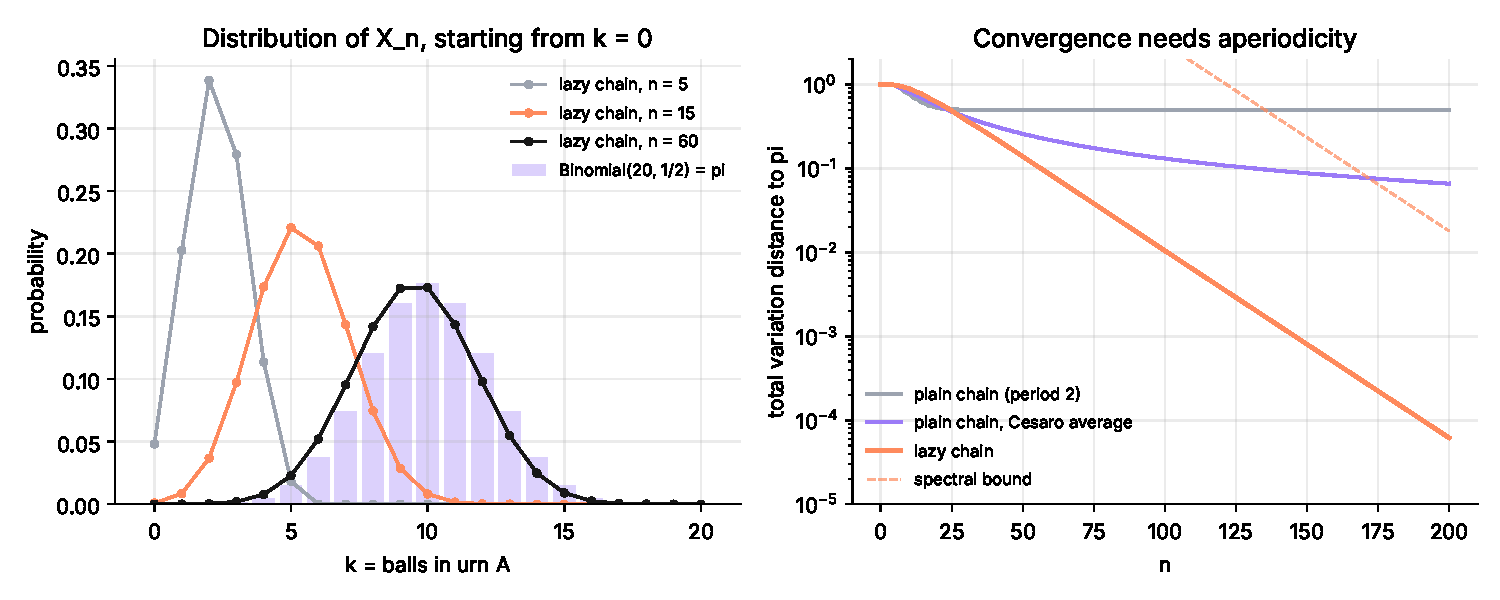
\includegraphics[width=\textwidth]{../figures/1_ehrenfest.pdf}
\caption{À gauche : loi de $X_n$ pour la chaîne paresseuse partant de $k = 0$ ; elle se rapproche de la binomiale. À droite : distance à l'équilibre. La chaîne d'Ehrenfest (période $2$) reste à distance $\frac12$, alors que les moyennes de Cesàro $\frac1n\sum_{k<n}\mu_k$ convergent ; la chaîne paresseuse converge géométriquement, sous la borne spectrale du théorème~\ref{thm:spectral}.}
\end{figure}

\section{Vitesse de convergence et trou spectral}

On mesure l'écart entre deux lois par la \emph{distance en variation totale}
\[
  \lVert \mu - \nu \rVert_\TV = \max_{A \subset E} |\mu(A) - \nu(A)| = \frac12 \sum_{i} |\mu_i - \nu_i| \in [0, 1].
\]
Pour une chaîne réversible, la vitesse de convergence se lit sur le spectre de $P$.

\begin{theoreme}[borne spectrale]\label{thm:spectral}
Soit $P$ irréductible et réversible par rapport à $\pi$. Ses valeurs propres sont réelles, $1 = \lambda_1 > \lambda_2 \ge \dots \ge \lambda_n \ge -1$ ; on note $\lambda_\star = \max(|\lambda_2|, |\lambda_n|)$. Pour tout état de départ $x$ et tout $t \ge 0$,
\[
  \lVert P^t(x, \cdot) - \pi \rVert_\TV \;\le\; \frac12 \sqrt{\frac{1 - \pi(x)}{\pi(x)}}\; \lambda_\star^{\,t}.
\]
\end{theoreme}

\begin{proof}
On munit $\R^E$ du produit scalaire $\langle f, g\rangle_\pi = \sum_x \pi(x) f(x) g(x)$. La réversibilité signifie exactement que $P$ (agissant sur les fonctions par $(Pf)(x) = \sum_y P_{xy} f(y)$) est autoadjoint :
\[
  \langle Pf, g\rangle_\pi = \sum_{x,y} \pi(x) P_{xy} f(y) g(x) = \sum_{x,y} \pi(y) P_{yx} f(y) g(x) = \langle f, Pg\rangle_\pi .
\]
Par le théorème spectral, il existe une base $\pi$-orthonormée de fonctions propres réelles $f_1 = \1, f_2, \dots, f_n$, avec $Pf_j = \lambda_j f_j$. Pour $y \in E$, la fonction $h_y = \1_{\{y\}}/\pi(y)$ a pour coordonnées $\langle h_y, f_j\rangle_\pi = f_j(y)$, donc $h_y = \sum_j f_j(y) f_j$ et
\[
  \frac{P^t(x,y)}{\pi(y)} = (P^t h_y)(x) = \sum_{j=1}^n \lambda_j^t f_j(x) f_j(y) = 1 + \sum_{j\ge2} \lambda_j^t f_j(x) f_j(y).
\]
À $x$ fixé, la fonction $u(y) = \frac{P^t(x,y)}{\pi(y)} - 1$ a donc les coordonnées $\lambda_j^t f_j(x)$ ($j \ge 2$), d'où
\[
  \lVert u\rVert_\pi^2 = \sum_{j\ge2} \lambda_j^{2t} f_j(x)^2 \le \lambda_\star^{2t} \sum_{j\ge2} f_j(x)^2 = \lambda_\star^{2t}\Big(\frac{1}{\pi(x)} - 1\Big),
\]
car $\sum_j f_j(x)^2 = \lVert h_x\rVert_\pi^2 = \pi(x)\cdot\pi(x)^{-2}$. Enfin, par Cauchy--Schwarz,
$2\lVert P^t(x,\cdot) - \pi\rVert_\TV = \sum_y \pi(y)\,|u(y)| \le \lVert u\rVert_\pi$.
\end{proof}

\begin{remarque}
La décroissance est asymptotiquement \emph{exactement} en $\lambda_\star^t$ dès que la composante de $h_x$ sur un vecteur propre associé est non nulle : la \emph{vitesse} de convergence est $\lambda_\star$, et le \emph{trou spectral} $1 - \lambda_\star$ la gouverne. Une valeur propre $-1$ (période $2$, comme pour Ehrenfest) empêche toute convergence.
\end{remarque}

\paragraph{Marche paresseuse sur un cycle.} Sur $\mathbb Z / m\mathbb Z$, on reste sur place avec probabilité $\frac12$ et l'on va sur chaque voisin avec probabilité $\frac14$. La loi uniforme est stationnaire et la chaîne est réversible.

\begin{proposition}
Les valeurs propres sont $\lambda_k = \frac{1 + \cos(2\pi k/m)}{2}$ pour $k = 0, \dots, m-1$. En particulier $\lambda_\star = \lambda_2 = \cos^2(\pi/m) = 1 - \frac{\pi^2}{m^2} + O(m^{-4})$.
\end{proposition}

\begin{proof}
La matrice est circulante : pour $\varphi_k(x) = e^{2i\pi kx/m}$, on a $(P\varphi_k)(x) = \frac12\varphi_k(x) + \frac14\big(\varphi_k(x+1) + \varphi_k(x-1)\big) = \big(\frac12 + \frac12\cos\frac{2\pi k}{m}\big)\varphi_k(x)$, et les $m$ fonctions $\varphi_k$ forment une base. Toutes ces valeurs propres sont positives, la plus grande après $1$ est obtenue pour $k = 1$, et $\frac{1+\cos 2\theta}{2} = \cos^2\theta$.
\end{proof}

Le temps de relaxation $1/(1-\lambda_\star) \approx m^2/\pi^2$ prédit que le temps de mélange $t_{\mathrm{mix}} = \min\{t : \lVert \mu_t - \pi\rVert_\TV \le \frac14\}$ croît comme $m^2$ : la marche se comporte comme une diffusion, qui met un temps de l'ordre de $m^2$ pour parcourir une distance $m$. Pour l'urne d'Ehrenfest, les valeurs propres sont $1 - \frac{2j}{N}$, $j = 0, \dots, N$ \cite{kac}, et celles de la chaîne paresseuse $1 - \frac jN$ ; donc $\lambda_\star = 1 - \frac1N$ (ces spectres sont vérifiés numériquement dans les tests).

\begin{table}[H]
\centering
\begin{tabular}{lccc}
\toprule
Chaîne & $\lambda_\star$ (théorie) & Taux observé & $t_{\mathrm{mix}}(1/4)$ \\
\midrule
\tableGap
\bottomrule
\end{tabular}
\caption{Le taux observé est la pente de $\log \lVert \mu_t - \pi\rVert_\TV$ en fonction de $t$, mesurée sur la fin de la décroissance (départ en un état fixé). Il coïncide avec la valeur propre théorique à $10^{-6}$ près.}
\end{table}

\begin{figure}[H]
\centering
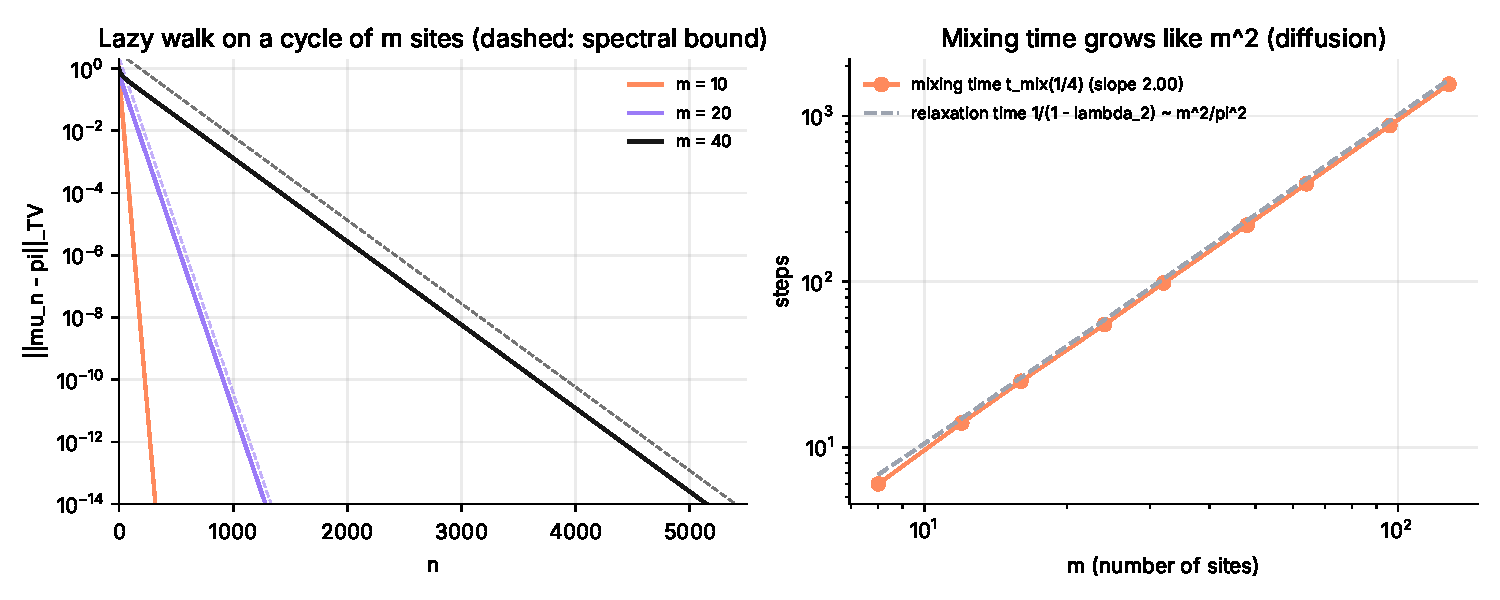
\includegraphics[width=\textwidth]{../figures/2_spectral_gap.pdf}
\caption{À gauche : distance à l'équilibre pour la marche sur un cycle, en trait plein, et borne du théorème~\ref{thm:spectral}, en pointillés : les pentes sont identiques. À droite : le temps de mélange suit une loi de puissance de pente \mixSlope{} en échelle log-log ($t_{\mathrm{mix}} = \mixHundred$ pour $m = 128$).}
\end{figure}

\section{Monte-Carlo : le théorème ergodique en pratique}\label{sec:mc}

Le théorème ergodique fournit une méthode de calcul par simulation, mais avec une erreur statistique. Un théorème central limite pour les chaînes de Markov (admis ici) prédit des fluctuations d'ordre $1/\sqrt n$ pour une trajectoire de longueur $n$. On simule en parallèle \nChains{} chaînes d'Ehrenfest indépendantes partant de $0$ et l'on moyenne la distance entre fréquences d'occupation et loi binomiale : la pente mesurée en échelle log-log est $\slopeErgodic$, conforme à la valeur théorique $-\frac12$ (figure~\ref{fig:mc}, à gauche). Pour gagner un chiffre de précision, il faut donc cent fois plus de pas : c'est pourquoi les méthodes déterministes sont préférables quand elles sont applicables, et pourquoi la simulation devient indispensable quand l'espace d'états est trop grand (section~\ref{sec:mcpr}).

\section{PageRank}

\subsection{Le surfeur aléatoire}

Brin et Page \cite{brin} ont proposé de classer les pages du Web par la fréquence avec laquelle un surfeur aléatoire les visite. Soit un graphe orienté pondéré à $n$ n\oe uds, de poids $w_{ij} > 0$ sur l'arc $i \to j$. La matrice des liens $S$ a pour coefficients $S_{ij} = w_{ij} / \sum_k w_{ik}$. Un n\oe ud sans arc sortant (\emph{n\oe ud pendant}) a une ligne nulle ; on la remplace par un vecteur de probabilité $v$ (uniforme par défaut), ce qui donne une matrice stochastique $S'$. À chaque étape, le surfeur suit un lien avec probabilité $\alpha$ (classiquement $0{,}85$) et se « téléporte » selon $v$ avec probabilité $1 - \alpha$ :
\[
  G = \alpha S' + (1-\alpha)\, \1 v^\top .
\]
\emph{PageRank} est la loi stationnaire $\pi$ de cette \emph{matrice de Google}. Si $v > 0$, tous les coefficients de $G$ sont strictement positifs : la chaîne est irréductible et apériodique, et le théorème~\ref{thm:fond} garantit l'existence et l'unicité de $\pi$.

\subsection{Convergence de la méthode de la puissance}

\begin{theoreme}\label{thm:pagerank}
Soit $x_0$ une loi de probabilité et $x_{k+1} = x_k G$. Alors
\[
  \lVert x_k - \pi\rVert_1 \le \alpha^k\, \lVert x_0 - \pi\rVert_1 \le 2\alpha^k
  \qquad\text{et}\qquad
  \lVert x_k - \pi\rVert_1 \le \frac{\lVert x_{k+1} - x_k\rVert_1}{1-\alpha}.
\]
\end{theoreme}

\begin{proof}
Si $x$ et $y$ sont deux lois de probabilité, $x\1 = y\1 = 1$ et donc $xG - yG = \alpha (x - y) S' + (1-\alpha)(x\1 - y\1) v^\top = \alpha (x-y) S'$. Or pour toute matrice stochastique $S'$ et tout vecteur ligne $z$,
$\lVert zS'\rVert_1 = \sum_j \big|\sum_i z_i S'_{ij}\big| \le \sum_i |z_i| \sum_j S'_{ij} = \lVert z\rVert_1$. Ainsi $\lVert xG - yG\rVert_1 \le \alpha\lVert x - y\rVert_1$ : $x \mapsto xG$ est contractante. Avec $y = \pi = \pi G$, on obtient $\lVert x_{k+1} - \pi\rVert_1 \le \alpha\lVert x_k - \pi\rVert_1$, d'où la première inégalité par récurrence. Pour la seconde, $\lVert x_k - \pi\rVert_1 \le \lVert x_k - x_{k+1}\rVert_1 + \lVert x_{k+1} - \pi\rVert_1 \le \lVert x_k - x_{k+1}\rVert_1 + \alpha\lVert x_k - \pi\rVert_1$.
\end{proof}

La seconde inégalité fournit un critère d'arrêt \emph{garanti} : on s'arrête quand $\lVert x_{k+1} - x_k\rVert_1 \le (1-\alpha)\,\varepsilon$, et l'erreur est alors inférieure à $\varepsilon$, sans connaître $\pi$. Le théorème entraîne aussi que toutes les valeurs propres de $G$ autres que $1$ sont de module au plus $\alpha$. Haveliwala et Kamvar \cite{haveliwala} ont montré que $|\lambda_2(G)| = \alpha$ exactement dès que $S'$ possède au moins deux classes fermées (des groupes de n\oe uds que l'on ne peut pas quitter en suivant les liens) : la borne en $\alpha^k$ est alors la vraie vitesse.

\paragraph{Mise en \oe uvre creuse.} On ne forme jamais $G$, qui est dense ($n^2$ coefficients). En notant $D$ l'ensemble des n\oe uds pendants,
\[
  xG = \alpha\, xS + \Big(\alpha \sum_{i\in D} x_i + (1-\alpha)\Big) v^\top ,
\]
et $xS$ se calcule en parcourant la liste des arcs : $(xS)_j = \sum_{i \to j} x_i S_{ij}$. Une itération coûte donc $O(\text{nombre d'arcs})$.

\subsection{Un estimateur de Monte-Carlo}\label{sec:mcpr}

\begin{proposition}
$\displaystyle \pi = (1-\alpha)\, v^\top (I - \alpha S')^{-1} = \sum_{k\ge0} (1-\alpha)\alpha^k\, v^\top S'^k$.
\end{proposition}

\begin{proof}
Comme $\pi\1 = 1$, l'équation $\pi = \pi G$ s'écrit $\pi = \alpha\pi S' + (1-\alpha) v^\top$, soit $\pi(I - \alpha S') = (1-\alpha)v^\top$. La matrice $I - \alpha S'$ est inversible et son inverse est la série de Neumann $\sum_k \alpha^k S'^k$, qui converge car $\lVert \alpha S'\rVert_\infty = \alpha < 1$.
\end{proof}

Interprétation : on lance un marcheur depuis un n\oe ud tiré selon $v$ ; à chaque étape, il s'arrête avec probabilité $1-\alpha$, sinon il fait un pas selon $S'$. Sa longueur $K$ suit la loi géométrique $\PP(K = k) = (1-\alpha)\alpha^k$, et sachant $K = k$, son point d'arrivée a pour loi $v^\top S'^k$. Par la proposition, \emph{le point d'arrivée suit exactement la loi $\pi$}. La fréquence des points d'arrivée de $N$ marches indépendantes est donc un estimateur sans biais de PageRank \cite{avrachenkov}, d'erreur en $1/\sqrt N$. Toutes les marches sont simulées simultanément (calcul vectoriel).

\section{Application : le réseau aérien mondial}

\subsection{Données}

Les données proviennent d'OpenFlights \cite{openflights} (liaisons aériennes à juin 2014, licence \emph{Open Database License}). Chaque aéroport est un n\oe ud ; l'arc $a \to b$ est pondéré par le nombre de compagnies qui exploitent la liaison. On obtient \nAirports{} aéroports, \nRoutes{} liaisons orientées et \nRouteEntries{} couples (compagnie, liaison) ; \nDangling{} aéroports n'ont aucun vol au départ. Le surfeur aléatoire devient un passager qui prend indéfiniment un vol au hasard depuis l'aéroport où il se trouve, en recommençant parfois son voyage d'un aéroport quelconque : PageRank mesure la proportion du temps qu'il passe dans chaque aéroport.

Le graphe a \nSCC{} composantes fortement connexes (calculées par l'algorithme de Kosaraju), dont une composante géante de \largestSCC{} aéroports, et \nClosed{} classes fermées de tailles \closedSizes{} : de petits réseaux régionaux (Nouvelle-Calédonie, Namibie, Alaska…) dont aucune liaison ne sort dans les données. D'après le résultat de Haveliwala et Kamvar, on a donc $|\lambda_2(G)| = \alpha$.

\subsection{Résultats et validation}

Avec $\alpha = 0{,}85$, la méthode de la puissance converge en \prIters{} itérations (erreur garantie $< 10^{-14}$) et \timeOurs~ms. La bibliothèque NetworkX, utilisée uniquement pour vérifier, donne les mêmes scores à $\diffNX$ près, en \timeNX~ms.

\begin{table}[H]
\centering
\small
\begin{tabular}{rllcc}
\toprule
Rang & Code & Ville (pays) & PageRank ($\times 1000$) & Rang par degré entrant \\
\midrule
\tableTop
\bottomrule
\end{tabular}
\caption{Les quinze aéroports de plus grand PageRank. Le degré entrant pondéré est le nombre de couples (compagnie, liaison) arrivant à l'aéroport.}
\end{table}

\begin{figure}[H]
\centering
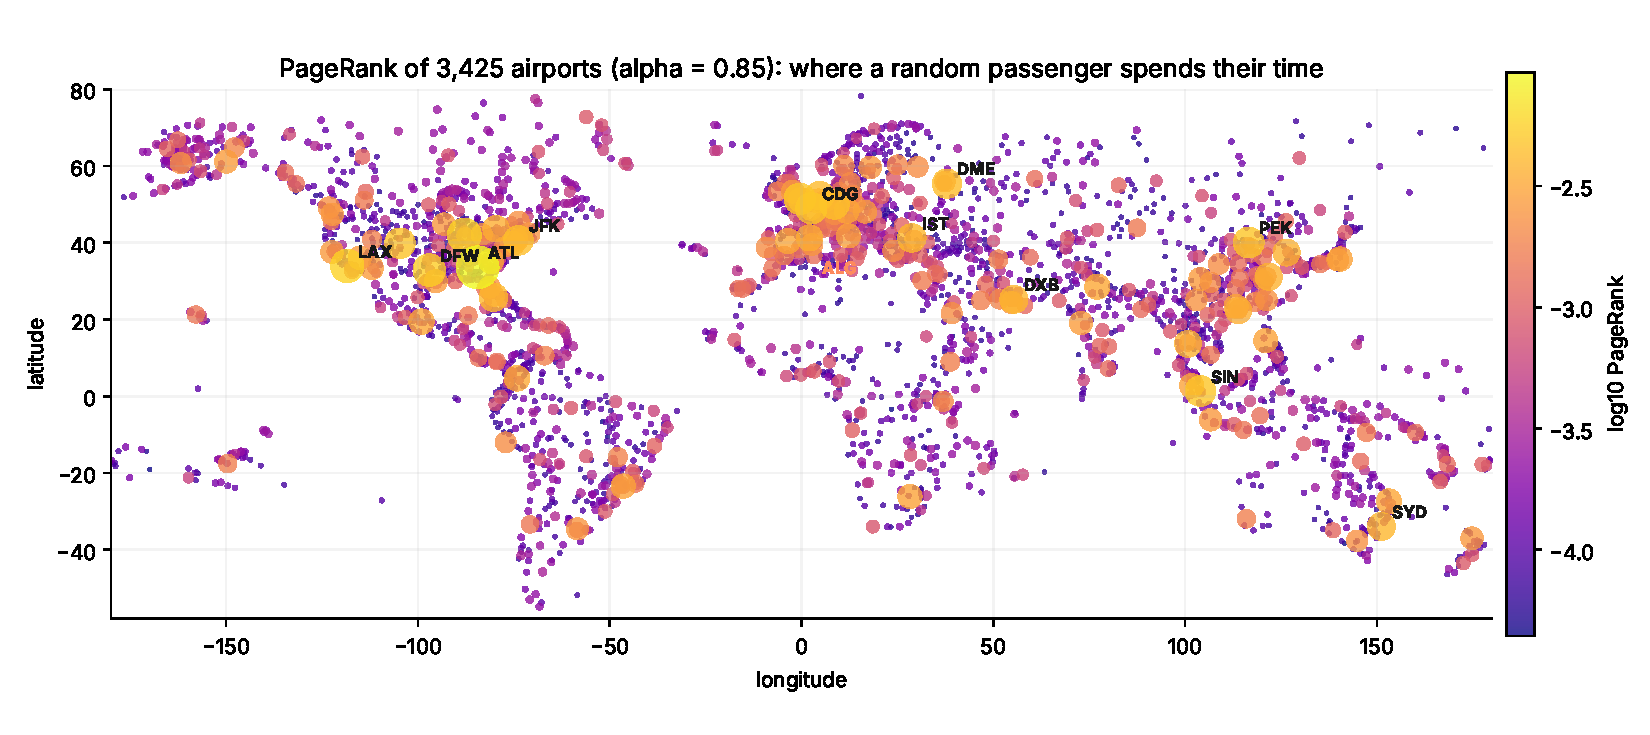
\includegraphics[width=\textwidth]{../figures/5_world_map.pdf}
\caption{Chaque aéroport est placé selon sa longitude et sa latitude ; taille et couleur indiquent son PageRank. Les grands hubs américains, européens et asiatiques dominent.}
\end{figure}

Le classement est très corrélé au nombre de liaisons entrantes (corrélation de rang de Spearman \spearmanDeg), mais il n'est pas identique : PageRank tient compte de \emph{l'importance} des aéroports d'où viennent les vols, et du temps que le passager passe dans une région. Les plus fortes progressions par rapport au degré concernent des réseaux régionaux denses et peu reliés au reste du monde :

\begin{table}[H]
\centering
\begin{tabular}{llcc}
\toprule
Code & Ville (pays) & Rang PageRank & Rang par degré entrant \\
\midrule
\tableUp
\bottomrule
\end{tabular}
\caption{Plus fortes progressions de rang parmi les cent premiers aéroports.}
\end{table}

L'Alaska en est l'exemple typique : un passager qui entre dans le réseau des petits aérodromes desservis depuis Anchorage, Fairbanks et Bethel y reste longtemps avant d'en ressortir, si bien que ces trois aéroports concentrent beaucoup de temps de présence. L'aéroport d'Alger (\texttt{ALG}) est au rang \algRank{} sur \nAirports{} (score $\algScore$, soit environ quatre fois et demie le score uniforme $\uniformScore$), contre le rang \algDegRank{} par degré entrant.

\begin{figure}[H]
\centering
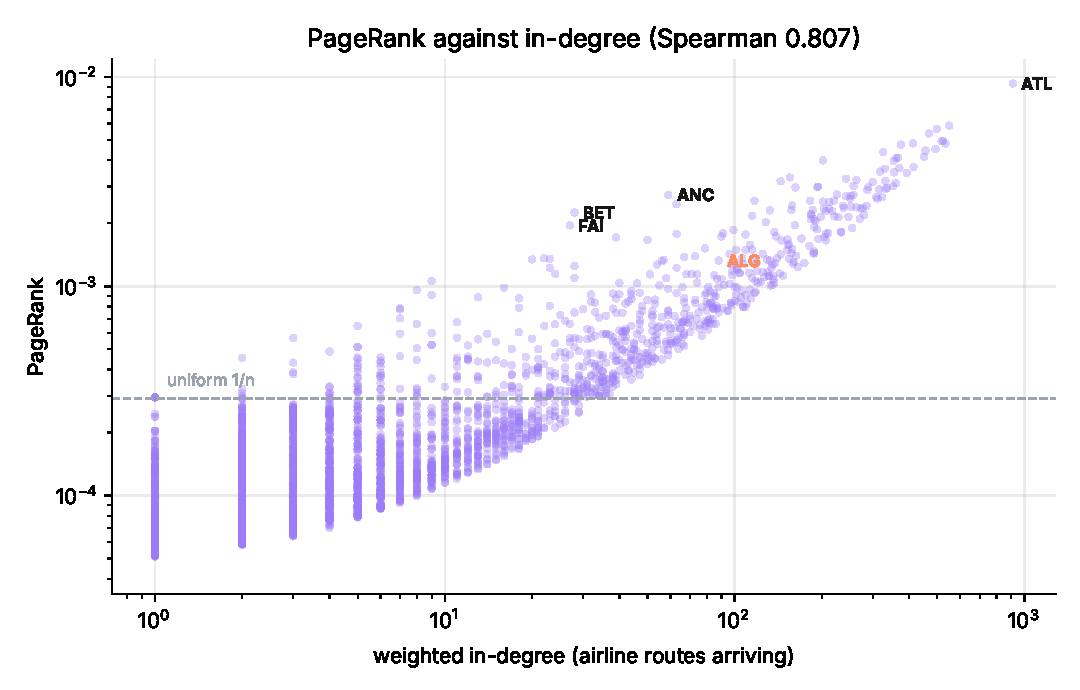
\includegraphics[width=0.78\textwidth]{../figures/6_pagerank_vs_degree.pdf}
\caption{PageRank en fonction du degré entrant pondéré. Les aéroports d'Alaska se détachent nettement au-dessus du nuage.}
\end{figure}

\subsection{Vitesse de convergence selon $\alpha$}

\begin{table}[H]
\centering
\begin{tabular}{cccc}
\toprule
$\alpha$ & Taux observé & Itérations pour $\lVert x_k - \pi\rVert_1 < 10^{-10}$ & Garanti par $\alpha^k\lVert x_0 - \pi\rVert_1$ \\
\midrule
\tableAlpha
\bottomrule
\end{tabular}
\caption{Départ uniforme. Le taux observé est toujours inférieur ou égal à $\alpha$ et s'en approche : il atteint $\alpha$ pour $\alpha = 0{,}99$, comme le prévoit l'existence de plusieurs classes fermées.}
\end{table}

\begin{figure}[H]
\centering
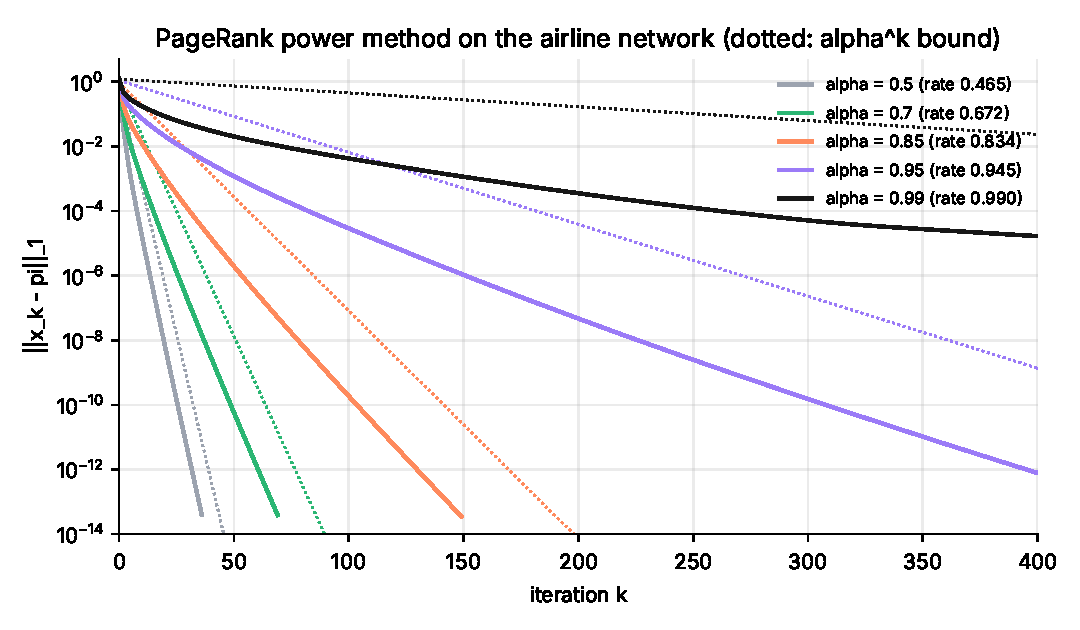
\includegraphics[width=0.8\textwidth]{../figures/4_convergence.pdf}
\caption{Erreur de la méthode de la puissance (trait plein) et borne $\alpha^k\lVert x_0 - \pi\rVert_1$ du théorème~\ref{thm:pagerank} (pointillés). Le nombre d'itérations est de l'ordre de $\log(1/\varepsilon) / \log(1/\alpha)$ : il explose quand $\alpha \to 1$.}
\end{figure}

Le choix de $\alpha$ est un compromis : proche de $1$, le modèle suit davantage la structure du graphe mais la convergence ralentit fortement, et le classement devient sensible aux classes fermées, qui finissent par absorber toute la masse. Avec $\alpha = 0{,}85$, il faut \itersEightyFive{} itérations pour une erreur de $10^{-10}$ (la borne en garantit \boundEightyFive), à environ \msPerIter~ms chacune.

\subsection{Estimation par Monte-Carlo}

\begin{table}[H]
\centering
\begin{tabular}{rcc}
\toprule
Marches & Erreur $\lVert \hat\pi - \pi\rVert_1$ & Temps (s) \\
\midrule
\tableMC
\bottomrule
\end{tabular}
\caption{Estimateur par les points d'arrivée de marches aléatoires ($\alpha = 0{,}85$), comparé à la méthode de la puissance.}
\end{table}

\begin{figure}[H]
\centering
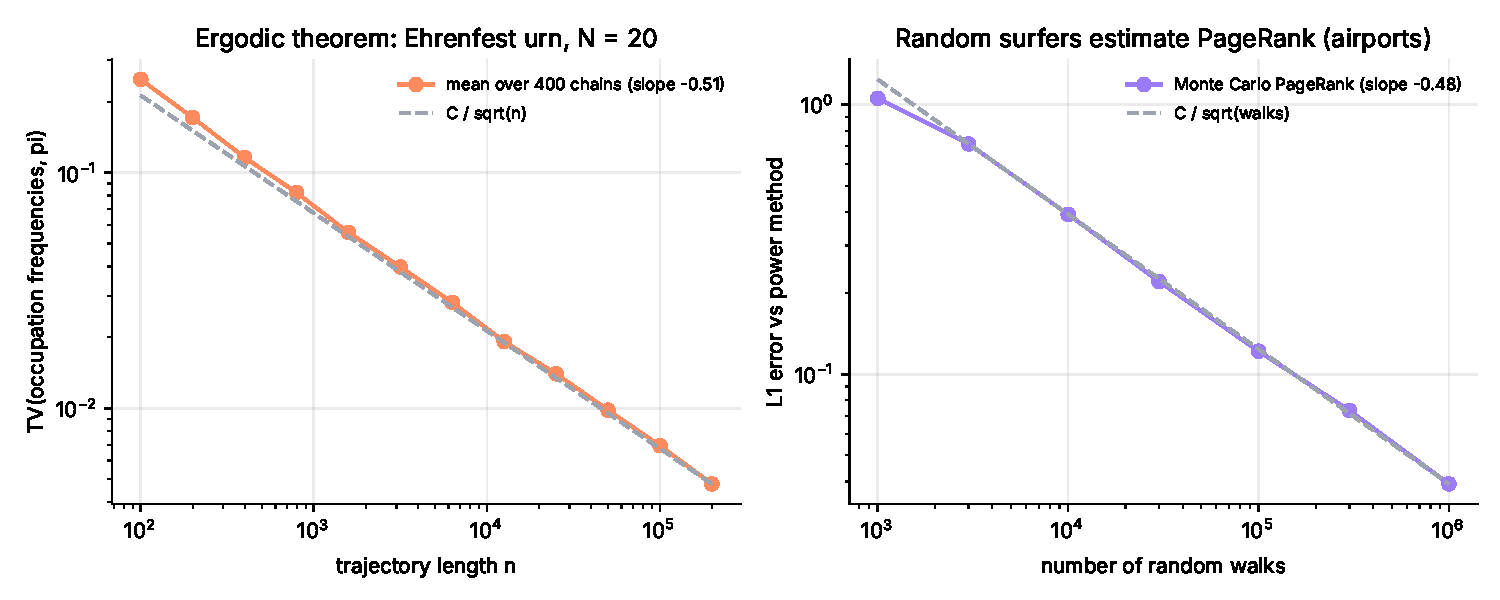
\includegraphics[width=\textwidth]{../figures/3_monte_carlo.pdf}
\caption{\label{fig:mc}Les deux estimateurs de Monte-Carlo convergent en $1/\sqrt n$ : pentes $\slopeErgodic$ pour le théorème ergodique (à gauche) et $\slopeMC$ pour PageRank (à droite).}
\end{figure}

L'erreur décroît avec une pente $\slopeMC$ (théorie : $-\frac12$). L'erreur totale reste importante ($\errMCmillion$ avec un million de marches) car elle cumule les erreurs sur les \nAirports{} aéroports, mais les scores élevés sont estimés précisément : les dix premiers aéroports estimés sont exactement les dix vrais (\sameTopTen{} sur 10). Cette propriété explique l'intérêt de la méthode pour les très grands graphes, où l'on cherche surtout les n\oe uds les plus importants \cite{avrachenkov}.

\section{Conclusion}

Les résultats théoriques sur les chaînes de Markov finies se vérifient avec précision : les trois calculs de la loi stationnaire concordent, la vitesse de convergence coïncide avec la deuxième valeur propre, le temps de mélange d'une marche sur un cycle croît comme le carré de sa taille, et les estimateurs de Monte-Carlo convergent en $1/\sqrt n$. Sur un réseau réel de plusieurs milliers de n\oe uds, une implémentation creuse de PageRank, guidée par la contraction en $\alpha$ démontrée plus haut, retrouve les résultats d'une bibliothèque de référence plus rapidement. Prolongements naturels : PageRank personnalisé (vecteur $v$ concentré sur un n\oe ud, pour mesurer la proximité à ce n\oe ud), l'algorithme HITS, et les méthodes de Monte-Carlo par chaînes de Markov (Metropolis--Hastings), qui construisent une chaîne de loi stationnaire donnée en imposant l'équilibre détaillé.

\begin{thebibliography}{9}
\bibitem{norris} J.~R. Norris, \emph{Markov Chains}, Cambridge University Press, 1997.
\bibitem{lpw} D.~A. Levin, Y. Peres, \emph{Markov Chains and Mixing Times}, 2\textsuperscript{e} éd. (avec E.~L. Wilmer), American Mathematical Society, 2017.
\bibitem{kac} M. Kac, Random walk and the theory of Brownian motion, \emph{American Mathematical Monthly} 54 (1947), 369--391.
\bibitem{brin} S. Brin, L. Page, The anatomy of a large-scale hypertextual Web search engine, \emph{Computer Networks and ISDN Systems} 30 (1998), 107--117.
\bibitem{langville} A.~N. Langville, C.~D. Meyer, \emph{Google's PageRank and Beyond}, Princeton University Press, 2006.
\bibitem{haveliwala} T.~H. Haveliwala, S.~D. Kamvar, The second eigenvalue of the Google matrix, rapport technique, Stanford University, 2003.
\bibitem{avrachenkov} K. Avrachenkov, N. Litvak, D. Nemirovsky, N. Osipova, Monte Carlo methods in PageRank computation: when one iteration is sufficient, \emph{SIAM Journal on Numerical Analysis} 45 (2007), 890--904.
\bibitem{openflights} OpenFlights, \emph{Airport and route databases}, \url{https://openflights.org/data.php}, licence Open Database License (ODbL).
\end{thebibliography}

\appendix
\section{Reproduire les résultats}

Le code, les tests et ce rapport sont disponibles sur GitHub. Toutes les valeurs numériques de ce document sont générées automatiquement :
\begin{verbatim}
pip install -r requirements.txt
python experiments/run_all.py     # figures, results.md et report/generated.tex
pytest                            # 26 tests
cd report && pdflatex rapport.tex && pdflatex rapport.tex
\end{verbatim}

\end{document}
